
\chapter{Introduction}
\label{chapter:intro}
\minitoc
\bigskip


% I like the introduction of the thesis of ZUCKER (but very short) : http://www.cs.cmu.edu/~mzucker/mz-thesis.pdf
\begin{figure}[h]
    \centering
    \captionsetup[subfigure]{justification=centering}
    \begin{subfigure}[t]{0.48\linewidth}
        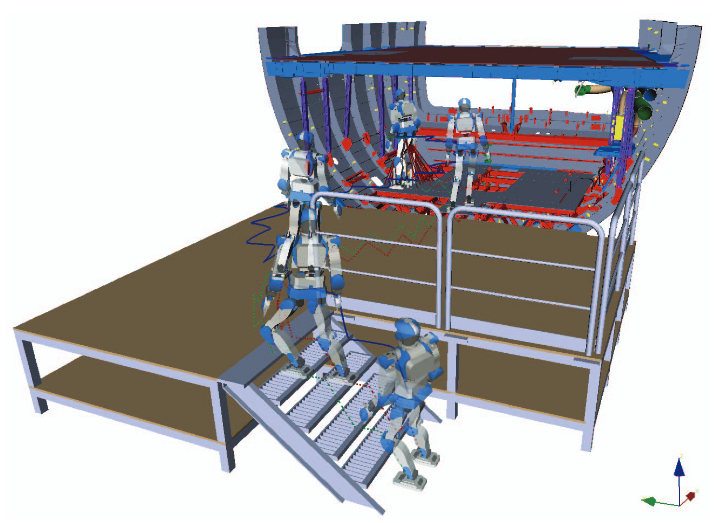
\includegraphics[width=\textwidth,height=5cm]{Figures/Chapter_INTRO/caron_image_plane.png}
        \caption{}
        \label{fig:intro_0}
    \end{subfigure}
    %\begin{subfigure}[t]{0.48\linewidth}
    %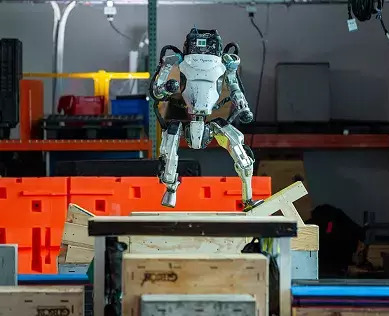
\includegraphics[width=\textwidth,height=5cm]{Figures/Chapter_INTRO/atlas_boston_dynamics.jpg}
    %\caption{\label{fig:intro_1}}
    %end{subfigure}
    \begin{subfigure}[t]{0.48\linewidth}
        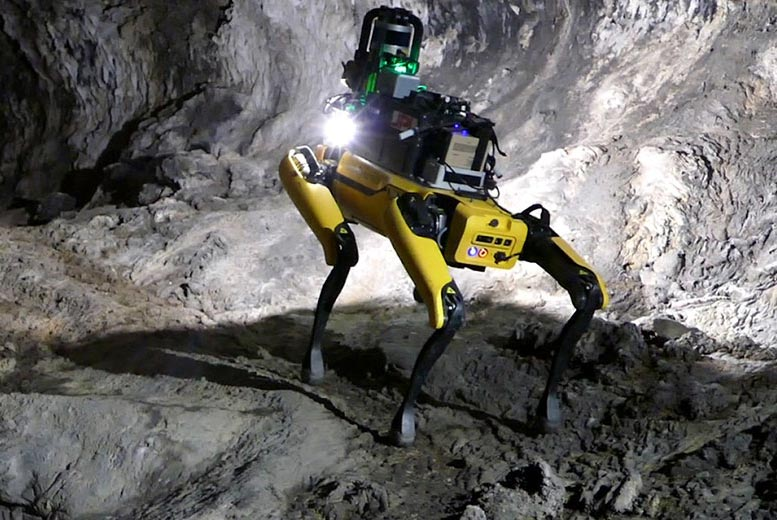
\includegraphics[width=\textwidth,height=4.5cm]{Figures/Chapter_INTRO/darpa_nasa.jpg}
        \caption{}
        \label{fig:intro_1}
    \end{subfigure}
    %\caption{Legged robots locomotion in complex environments. Sources: (a) \copyright Boston Dynamics and (b) \copyright NASA/JPL-Caltech.\label{fig:intro}}
    %\caption{Legged robots locomotion in complex environments. Sources: Caron et al. \cite{caron_plane_2016} and (b) ATLAS robot \copyright Boston Dynamics.\label{fig:intro}}
    \caption{Legged robots locomotion in complex environments. Sources: Caron et al. \cite{caron_plane_2016} and (b) \copyright NASA/JPL-Caltech.}
    \label{fig:intro}
\end{figure}

% TITLE: Reinforcement Learning of a Navigation Method for Contact Planning on Humanoid Robots


%    What is the problem?
%    Why is it interesting and important?
%    Why is it hard? (E.g., why do naive approaches fail?)
%    Why hasn't it been solved before? (Or, what's wrong with previous proposed solutions? How does mine differ?)
%    What are the key components of my approach and results? Also include any specific limitations. 

% https://www.futura-sciences.com/tech/actualites/robotique-interview-construire-robots-humanoides-90953/ : 
% Un des principaux intérêts motivant la construction de robots humanoïdes est sans doute sa compatibilité avec le monde des humains. Sans adaptation de notre environnement, ils pourraient vivre en harmonie avec nous au quotidien pour nous aider et utiliser nos infrastructures.

Robots are already essential tools in the industry. 
However, most of them require a specifically designed environment to perform repetitive tasks for manufacturing.
In recent years, research on legged robots has opened a whole new range of possibilities. %in primarily human-made environments.
These robots could operate in industrial areas and perform various tasks just like humans, or explore in our stead risky environments (Figure \ref{fig:intro}).
Nevertheless, to do so, they have to perform the most basic but challenging skill that is to \textit{locomote through the environment}.

\section{Legged locomotion in complex environments}
% Je veux refaire le raisonnement de ce qu'un humain fait pour se mouvoir.
\begin{figure}[h]
    \centering
    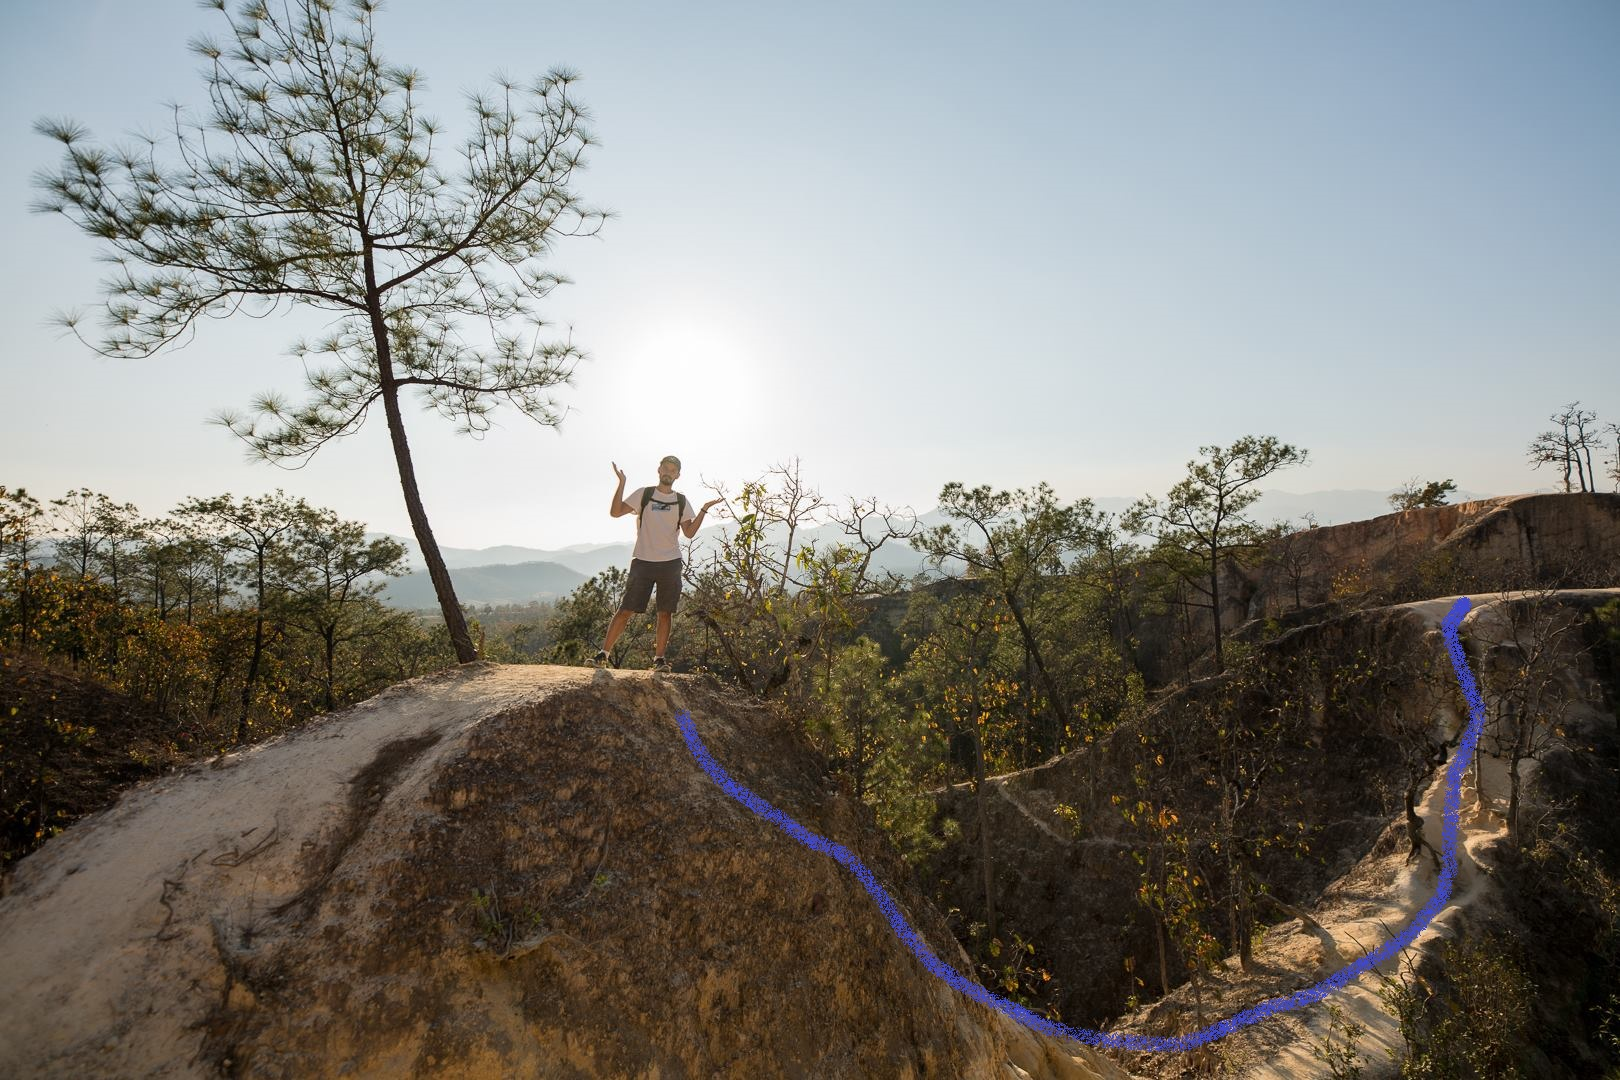
\includegraphics[width=\textwidth, height=8cm, trim={10cm 0 0 8cm}, clip]{Figures/Chapter_INTRO/moi_chemin.jpg}
    \caption{Planning the path and contacts is crucial to locomote on complex terrains.}
    \label{fig:intro:moi_chemin}
\end{figure}
In the large collection of works on legged robots, several strategies emerged to solve this problem.
In this thesis, we are interested in the locomotion of these robots in complex environments, that can operate with a similar decision process to their creators.

We humans can achieve this task in real-time. 
As shown in Figure \ref{fig:intro:moi_chemin}, the problem I have to solve is as follows: \qq{how can I reach the other side of this terrain?}
Here, this task is particularly difficult and so thorough planning is required.
I can typically decompose this task into two sub-problems:
\begin{enumerate}
    \item \textit{What path do I take?} 
    This decision is based on an estimation of my capabilities. 
    First, the path is subject to conditions of \textit{reachability}, as I need to be able to touch the ground along the path, and of \textit{collision-avoidance}. 
    Second, I need to evaluate the terrain \textit{traversability} to plan a feasible path. Based on these criteria, I am going to follow the blue path in our example.
    \item \textit{How to follow the path with my body?} 
    While walking without thinking where to place my foot could be sufficient for most scenarios, difficult scenes such as this one require a careful \textit{contact planning} for me to avoid taking a wrong step and falling.
\end{enumerate}
Human locomotion typically performs these two stages with (1) a navigation task to plan a feasible path up to our objective, and (2) walking along this path while carefully planning our contact on the terrain.

Legged robot locomotion in general can benefit from these stages as demonstrated during the DARPA subterranean challenge \cite{darpa_nasa_2021, darpa_hutter_2022}.
In disaster scenarios, these robots have to map, navigate, and search for casualties in complex underground environments.

However, reproducing the masterful human reasoning for locomotion is yet a difficult problem. How to program robots to achieve a similar decision process?
Furthermore, this decision process changes from individual to individual who continuously learns to estimate and improve their capabilities.



\section{Thesis Statement and Summary.}

We aim for a fast to compute and safe solution for legged robot locomotion in complex environments.
For that, we further explored the use of a navigation task prior to planning contacts on the terrain.
Our research topic is the critical limitation of this approach, that is the path feasibility by a contact planner.

Our main contribution is a local navigation method learned by reinforcement. 
Our method, named LEAS, can locally navigate the terrain under reachability and collision-avoidance constraints using a local height map.
During training time, LEAS can be plugged into a contact planner to learn how to generate more likely feasible paths for it.
Finally, we tested our method with 3 different contact planners from the Loco3D project \cite{loco3d}.

The organization of this thesis is as follows:

Chapter \ref{sec:sota} presents a review of the works on legged robot locomotion. 
We explore different solutions to obtain a safe and robust locomotion, leading us to our choice of a navigation method prior to contact planning (also known as the motion-before-contact approach). Finally, we present a general literature overview of the methods used in navigation that inspired our solution.

Chapter \ref{sec:LEAS} presents in-depth our steering method LEAS, that can locally navigate complex terrains.
We first describe the environment implemented to learn by reinforcement how to generate guide paths under reachability and collision-avoidance constraints.
This chapter presents LEAS without being plugged into a contact planner, which is a local navigation task in 3D.

Chapter \ref{sec:CP-SB} presents the results of LEAS plugged into the acyclic sampling-based contact planner \cite{AcyclicCP}. 
Our steering method learns how to generate guide paths fitting this contact planner. 
As a result, it solves the compatibility problem we had with our previous solutions between navigation and contact planning.

Chapter \ref{sec:CP-SL1M} investigates the use of LEAS plugged into the Mixed-Integer Programming contact planner and its relaxation \cite{sl1m_v2}. 
We explain the formulations of these contact planners and their limitations relative to the guide. Finally, we present the results as well as the different experiments we conducted.

Chapter \ref{sec:conclusion} discusses the advantages and limitations of our steering method. Finally, we conclude with the perspective of this work.